\documentclass[10pt,a4paper]{scrartcl}
\pagestyle{empty}
\usepackage{a4} % alternativ \usepackage{a4wide}
\usepackage[ngerman]{babel} % Neudeutsche Silbentrennung (mehrsprachiges Dokument)
\usepackage{parskip} % Skip indentation of first row
\usepackage{graphicx} % Graphics support
\usepackage{longtable} % Tables across several pages
\usepackage{booktabs}
\usepackage{hyperref} % Hyperlinks
\usepackage[automark]{scrpage2} %kopf/fusszeile
\usepackage[utf8x]{inputenc} % Unicode-Encoding
 
\linespread{1.3}

\author{Danilo Bargen, Christian Fässler, Jonas Furrer} 
\title{Externes Design\\ Projekt BierIdee}

\pagestyle{scrheadings}
\ihead{SE2 Projekte} %linke Kopfzeile
\ohead{BierIdee} %rechte Kopfzeile

\begin{document}

\begin{titlepage}
	\maketitle
	\vspace{120mm}
	\thispagestyle{empty} % Don't start page numbers on this page
\end{titlepage}

\tableofcontents
\newpage

\section*{Änderungshistorie}
\begin{tabular}{p{0.1\textwidth}p{0.15\textwidth}p{0.55\textwidth}p{0.1\textwidth}}
\toprule
\textbf{Version} & \textbf{Datum} & \textbf{Änderung} & \textbf{Person} \\  
\midrule
v1.0 & 07.05.2012 & Dokument erstellt & jfurrer \\  
\bottomrule
\end{tabular} 
\newpage

\section{Mockup Skizzen}
Folgende Skizzen sind die Basis für das externe Design der BierIdee App.
\subsection{Login}
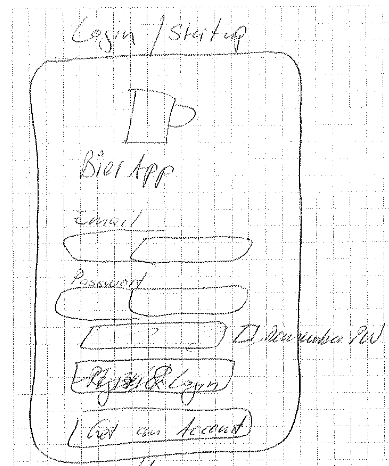
\includegraphics[scale=.5]{login-skizze.png}

\subsection{Registrierung}
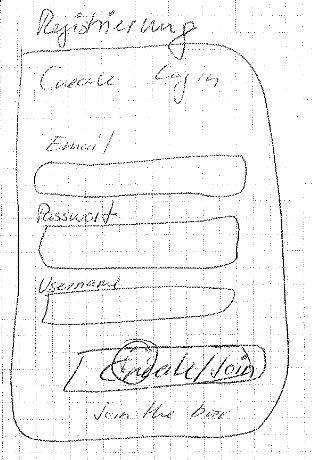
\includegraphics[scale=.5]{registrierung-skizze.png}

\subsection{Home/Dashboard}
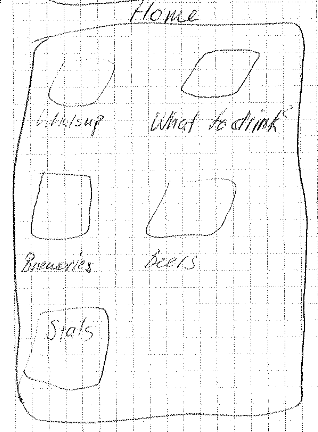
\includegraphics[scale=.5]{home-skizze.png}
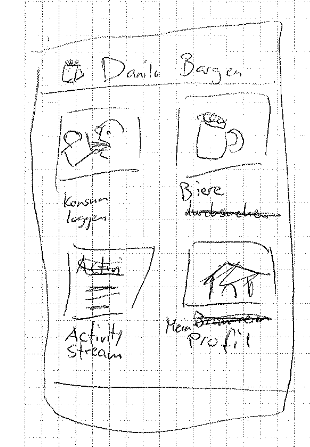
\includegraphics[scale=.5]{home-skizze-2.png}

\subsection{Beerdetail}
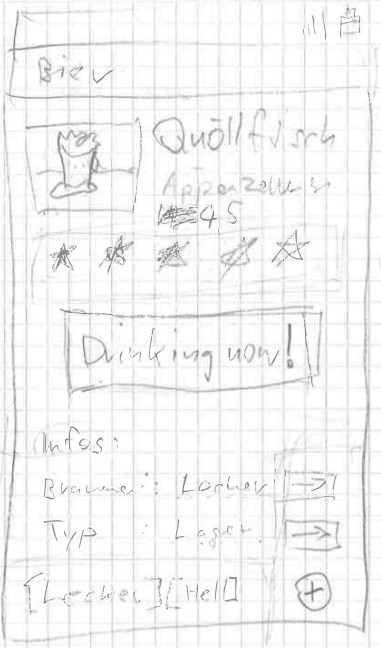
\includegraphics[scale=.5]{bierdetail-skizze.png}

\section{Mockup Screens}
Folgene Screens zeigen die momentane Ausprägung der entsprechenden Activities.
\subsection{Login}
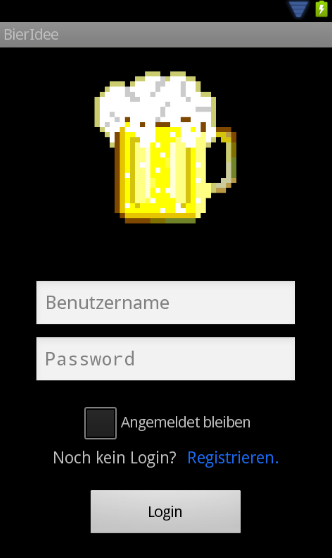
\includegraphics[scale=.35]{login-screen.png}

\subsection{Registrierung}
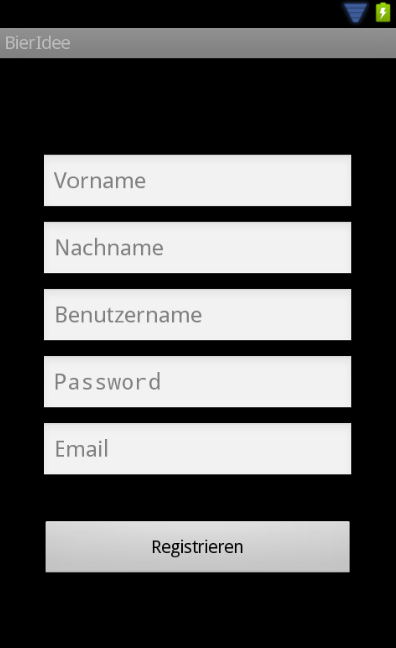
\includegraphics[scale=.3]{registrierung-screen.png}

\subsection{Home/Dashboard}
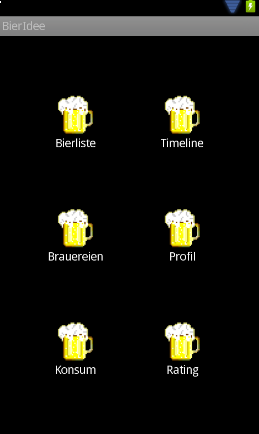
\includegraphics[scale=.5]{home-screen.png}

\subsection{Beerdetail}
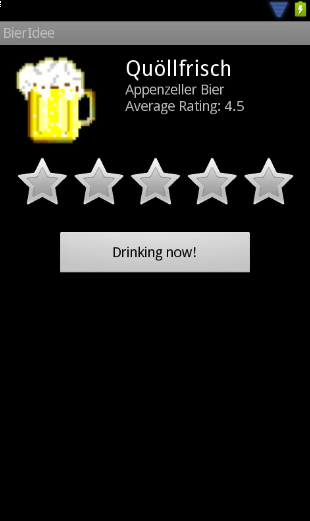
\includegraphics[scale=.4]{bierdetail-screen.png}

\end{document}
